\documentclass[11pt,twocolumn,oneside,openany,headings=optiontotoc,11pt,numbers=noenddot]{article}

\usepackage[a4paper]{geometry}
\usepackage[utf8]{inputenc}
\usepackage[T1]{fontenc}
\usepackage{lmodern}
\usepackage[ngerman]{babel}
\usepackage{ngerman}

\usepackage[onehalfspacing]{setspace}

\usepackage{fancyhdr}
\usepackage{fancybox}

\usepackage{rotating}
\usepackage{varwidth}

%Struktogramme
\usepackage[german,curves]{struktex}

\usepackage{pdflscape}
\usepackage{changepage}
\usepackage{graphicx}
\usepackage[bottom]{footmisc}
\usepackage{transparent}
\usepackage{graphbox}
\graphicspath{
	{Pics/PDFs/}
	{Pics/JPGs/}
	{Pics/PNGs/}
}
\usepackage{caption}
\usepackage{wrapfig}
\usepackage{marginnote}
\usepackage{tabularx}
\usepackage{dashrule}
\usepackage{soulutf8}
\usepackage{hhline}
%arydshln suppresses vertical lines in table
%\usepackage{arydshln}
\usepackage{multirow}
\usepackage{enumerate}
\usepackage[hidelinks]{hyperref}
\usepackage{listings}

\usepackage[table]{xcolor}
\usepackage{array}
\usepackage{enumitem,amssymb,amsmath}
\usepackage{interval}
\usepackage{cancel}
\usepackage{stmaryrd}
\usepackage{wasysym}
\usepackage{polynom}
\usepackage{diagbox}
\usepackage{dashrule}
\usepackage{framed}
\usepackage{mdframed}
\usepackage{karnaugh-map}
\usepackage{pdfpages}

\usepackage{blindtext}

\usepackage{eso-pic}

\usepackage{amssymb}
\usepackage{eurosym}

\usepackage[pages=some]{background}
\pagestyle{headings}
\renewcommand{\headrulewidth}{0.2pt}
\renewcommand{\footrulewidth}{0.2pt}
\newcommand*{\underdownarrow}[2]{\ensuremath{\underset{\overset{\Big\downarrow}{#2}}{#1}}}
\setlength{\fboxsep}{5pt}
\newcommand{\explainBelow}[3]{\underbrace{#1}_{\parbox{\widthof{#3}}{\footnotesize\raggedright #2}}}
\newcommand{\explainAbove}[3]{\overbrace{#1}^{\parbox{\widthof{#3}}{\footnotesize\raggedright #2}}}
\newcommand\footnoteref[1]{\protected@xdef\@thefnmark{\ref{#1}}\@footnotemark}


% Codestyle defined
\definecolor{codegreen}{rgb}{0,0.6,0}
\definecolor{codegray}{rgb}{0.5,0.5,0.5}
\definecolor{codepurple}{rgb}{0.58,0,0.82}
\definecolor{backcolour}{rgb}{0.95,0.95,0.92}
\definecolor{deepgreen}{rgb}{0,0.5,0}
\definecolor{darkblue}{rgb}{0,0,0.65}
\definecolor{mauve}{rgb}{0.40, 0.19,0.28}
\colorlet{exceptioncolour}{yellow!50!red}
\colorlet{commandcolour}{blue!60!black}
\colorlet{numpycolour}{blue!60!green}
\colorlet{specmethodcolour}{violet}

%Neue Spaltendefinition
\newcolumntype{L}[1]{>{\raggedright\let\newline\\\arraybackslash\hspace{0pt}}m{#1}}
\newcolumntype{M}{>{\centering\arraybackslash}X}
\newcommand{\cmnt}[1]{\ignorespaces}
%Textausrichtung ändern
\newcommand\tabrotate[1]{\rotatebox{90}{\raggedright#1\hspace{\tabcolsep}}}

%Intervall-Konfig
\intervalconfig {
	soft open fences
}

%Bash
\lstdefinestyle{BashInputStyle}{
	language=bash,
	basicstyle=\small\sffamily,
	backgroundcolor=\color{backcolour},
	columns=fullflexible,
	backgroundcolor=\color{backcolour},
	breaklines=true,
}
%Java
\lstdefinestyle{JavaInputStyle}{
	language=Java,
	backgroundcolor=\color{backcolour},
	aboveskip=1mm,
	belowskip=1mm,
	showstringspaces=false,
	columns=flexible,
	basicstyle={\footnotesize\ttfamily},
	numberstyle={\tiny},
	numbers=none,
	keywordstyle=\color{purple},,
	commentstyle=\color{deepgreen},
	stringstyle=\color{blue},
	emph={out},
	emphstyle=\color{darkblue},
	emph={[2]rand},
	emphstyle=[2]\color{specmethodcolour},
	breaklines=true,
	breakatwhitespace=true,
	tabsize=2,
}
%Python
\lstdefinestyle{PythonInputStyle}{
	language=Python,
	alsoletter={1234567890},
	aboveskip=1ex,
	basicstyle=\footnotesize,
	breaklines=true,
	breakatwhitespace= true,
	backgroundcolor=\color{backcolour},
	commentstyle=\color{red},
	otherkeywords={\ , \}, \{, \&,\|},
	emph={and,break,class,continue,def,yield,del,elif,else,%
		except,exec,finally,for,from,global,if,import,in,%
		lambda,not,or,pass,print,raise,return,try,while,assert},
	emphstyle=\color{exceptioncolour},
	emph={[2]True,False,None,min},
	emphstyle=[2]\color{specmethodcolour},
	emph={[3]object,type,isinstance,copy,deepcopy,zip,enumerate,reversed,list,len,dict,tuple,xrange,append,execfile,real,imag,reduce,str,repr},
	emphstyle=[3]\color{commandcolour},
	emph={[4]ode, fsolve, sqrt, exp, sin, cos, arccos, pi,  array, norm, solve, dot, arange, , isscalar, max, sum, flatten, shape, reshape, find, any, all, abs, plot, linspace, legend, quad, polyval,polyfit, hstack, concatenate,vstack,column_stack,empty,zeros,ones,rand,vander,grid,pcolor,eig,eigs,eigvals,svd,qr,tan,det,logspace,roll,mean,cumsum,cumprod,diff,vectorize,lstsq,cla,eye,xlabel,ylabel,squeeze},
	emphstyle=[4]\color{numpycolour},
	emph={[5]__init__,__add__,__mul__,__div__,__sub__,__call__,__getitem__,__setitem__,__eq__,__ne__,__nonzero__,__rmul__,__radd__,__repr__,__str__,__get__,__truediv__,__pow__,__name__,__future__,__all__},
	emphstyle=[5]\color{specmethodcolour},
	emph={[6]assert,range,yield},
	emphstyle=[6]\color{specmethodcolour}\bfseries,
	emph={[7]Exception,NameError,IndexError,SyntaxError,TypeError,ValueError,OverflowError,ZeroDivisionError,KeyboardInterrupt},
	emphstyle=[7]\color{specmethodcolour}\bfseries,
	emph={[8]taster,send,sendMail,capture,check,noMsg,go,move,switch,humTem,ventilate,buzz},
	emphstyle=[8]\color{blue},
	keywordstyle=\color{blue}\bfseries,
	rulecolor=\color{black!40},
	showstringspaces=false,
	stringstyle=\color{deepgreen}
}

\lstset{literate=%
	{Ö}{{\"O}}1
	{Ä}{{\"A}}1
	{Ü}{{\"U}}1
	{ß}{{\ss}}1
	{ü}{{\"u}}1
	{ä}{{\"a}}1
	{ö}{{\"o}}1
}

% Neue Klassenarbeits-Umgebung
\newenvironment{worksheet}[3]
% Begin-Bereich
{
	\newpage
	\sffamily
	\setcounter{page}{1}
	\ClearShipoutPicture
	\AddToShipoutPicture{
		\put(55,761){{
				\mbox{\parbox{385\unitlength}{\tiny \color{codegray}BBS I Mainz, #1 \newline #2
						\newline #3
					}
				}
			}
		}
		\put(455,761){{
				\mbox{\hspace{0.3cm}
\includegraphics[width=0.2\textwidth]{../../logo.pdf}}
			}
		}
	}
}
% End-Bereich
{
	\clearpage
	\ClearShipoutPicture
}

\setlength{\columnsep}{3em}
\setlength{\columnseprule}{0.5pt}

\geometry{left=2.50cm,right=2.50cm,top=3.00cm,bottom=1.00cm,includeheadfoot}
\pagenumbering{gobble}
\pagestyle{empty}

\begin{document}
	\begin{worksheet}{Berufliches Gymnasium}{Klassenstufe 13 - Mathematik}{Lernabschnitt 2: Binomialverteilung}
		\setcounter{section}{1}
		\section{Die Binomialverteilung}
		\subsection{Das Bernoulli-Experiment}
		Viele Zufallsexperimente weisen folgende Standardform auf:\\
		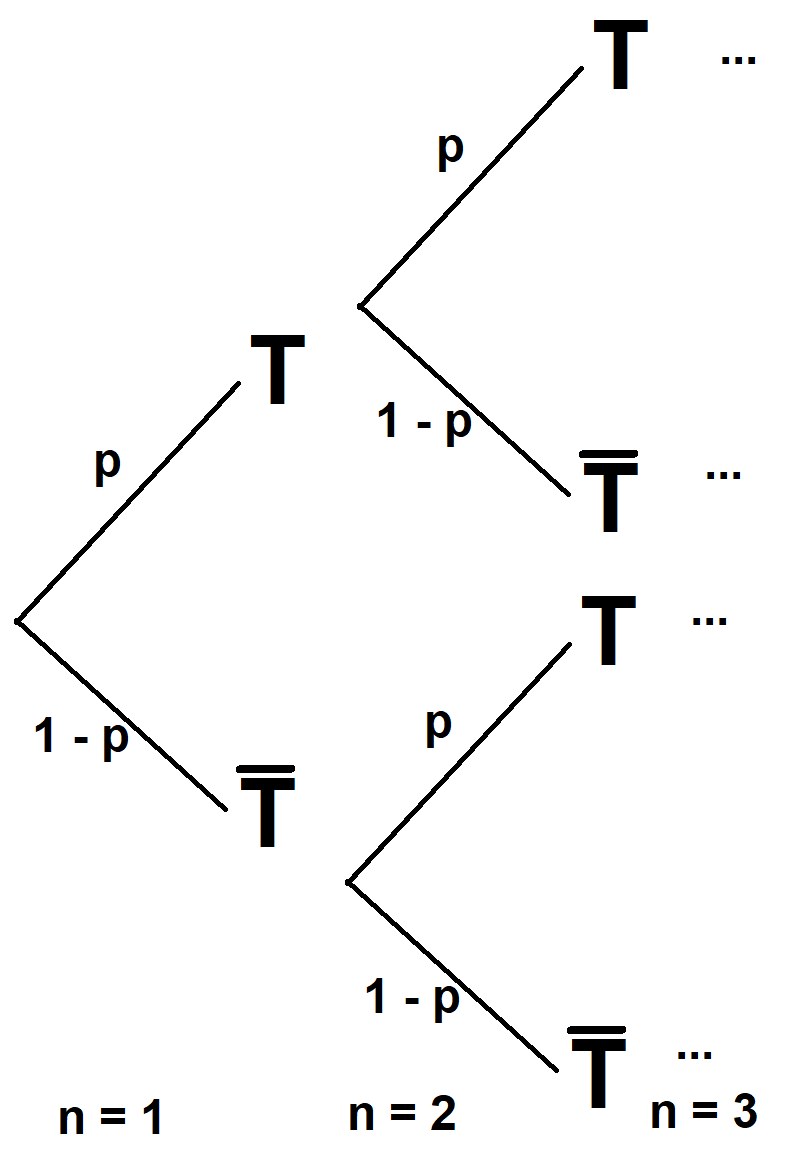
\includegraphics[width=0.48\textwidth]{../99_Bilder/04_WKR/bern.png}\\
		\textit{Symbolik/Begriffe}:\\
		\(T\): \grqq{}Treffer\grqq{} per Definition\\
		\(\overline{T}\): Gegenereignis zu \grqq{}Treffer\grqq{}\\
		p: Wahrscheinlichkeit eines Treffers\\
		n: gesamte Anzahl der Stufen\\
		\par\noindent
		Bei einem solchen Experiment ist es von großer Bedeutung, dass man vor jeglicher Analyse festlegt, was als Treffer gilt, welche Bedeutung die Stufen haben und natürlich welche Wahrscheinlichkeiten vorliegen.
		\begin{framed}
			\noindent
			In einem \textbf{Bernoulli-Experiment} gibt es auf jeder Stufe nur zwei mögliche Ausgänge.\\
			Die Bedeutung bzw. Zuordnung der Äste ändert sich zwischen den Stufen nicht.\\
			Die Wahrscheinlichkeit bleibt von Stufe zu Stufe gleich. Heißt, ein Ergebnis auf einer Stufe hat keine Auswirkungen auf die Wahrscheinlichkeit der nächsten Stufe.
		\end{framed}
		Die Ereignisse eines Bernoulli-Zufallsexperiments können für die \glqq{}Anzahl der Treffer\grqq{} stehen. Somit kann folgende Zufallsvariable festgelegt werden:\\
		\par\noindent
		\renewcommand{\arraystretch}{1.5}
		\begin{tabularx}{0.48\textwidth}{|l|M|M|M|M|}
			\hline
			\(x_i\) & 0 & 1 & $\ldots$ & n\\
			\hline
			\(P(X = x_i)\) & & & &\\
			\hline
		\end{tabularx}\\
		\par\noindent
		Haben wir eine solche \textbf{Wahrscheinlichkeitsverteilung}, so sprechen wir von einer \textbf{\underline{Binomialverteilung}}.\\
		\subsubsection*{Beispiel: LRS}
		\begin{framed}
			\noindent
			Der Anteil von Kindern mit Lese- und Rechtschreibschwäche (LRS) liegt in der BRD bei 10\%. Der Wert kann als Wahrscheinlichkeit dafür interpretiert werden, dass bei einem Kind im Laufe der Grundschulzeit LRS festgestellt wird.\\
			In eine Grundschule werden 50 Kinder eingeschult.
		\end{framed}
		Wir definieren wie folgt:\\
		\(T\): Kind hat eine LRS\\
		\(\overline{T}\): Kind hat keine LRS\\
		p: \(0,10\) (empirische Wahrscheinlichkeit)\\
		\(n = 50\)\\
		\par\noindent
		\textit{Gesucht}: Anzahl der Kinder mit einer LRS
		\subsection{Die Wahrscheinlichkeiten bei der Binomialverteilung}
		Die Wahrscheinlichkeit bei der Binomialverteilung lassen sich durch folgende Formeln  ermitteln:
		\begin{align*}
			P(X=k) = \binom{n}{k}\cdot{}p^n\cdot(1-p)^{n-k}
		\end{align*}
		Dabei gibt \(\binom{n}{k}\) die Anzahl der Pfade an.\\
		\(p^n\cdot(1-p)^{n-k}\) entspricht der Wahrscheinlichkeit eines beliebigen zum Ereignis \(X = k\) gehörenden Pfades (\grqq{}Pfadregel\grqq{}).
		\subsubsection{Tabellen zur Binomialverteilung}
		Damit man nicht jedes Mal in die Formel einsetzen muss, existieren Tabellen, bei denen man für eine bestimmte Anzahl Stufen und Trefferwahrscheinlichkeiten die Wahrscheinlichkeiten für die Ereignisse \(X = k\) ablesen kann.\\
		\par\noindent
		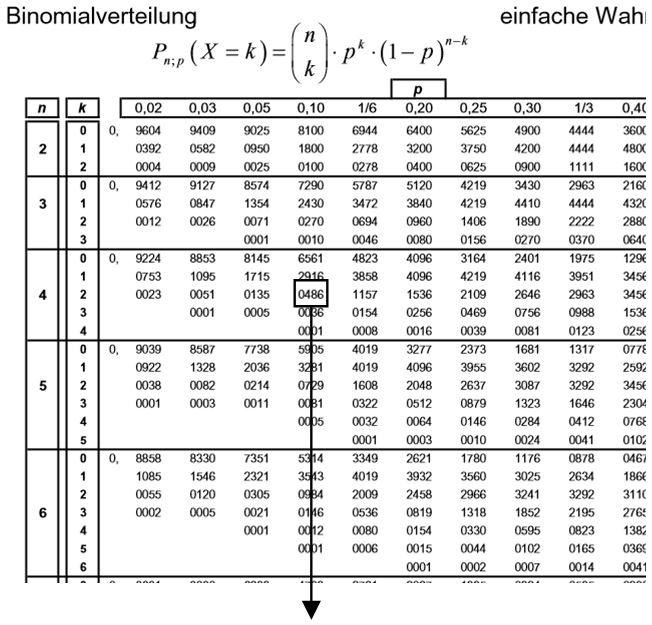
\includegraphics[width=0.48\textwidth]{../99_Bilder/04_WKR/binomtab.jpg}\\
		\underline{Beispiel:} Die Wahrscheinlichkeit, dass es bei einem vierstufigen Bernoulli-Experiment mit einer Trefferwahrscheinlichkeit von \(0,10\) zu \underline{genau} 2 Treffern kommt, liegt bei \(0,0486\).\\
		\par\noindent
		Meist liegt eine Tabelle zur \underline{kumulierten Binomialverteilung} vor. Diese gibt die Wahrscheinlichkeit für Ereignisse wie \(X < k\ (X = {0, 1, 2, \ldots, k})\) an.\\
		\par\noindent
		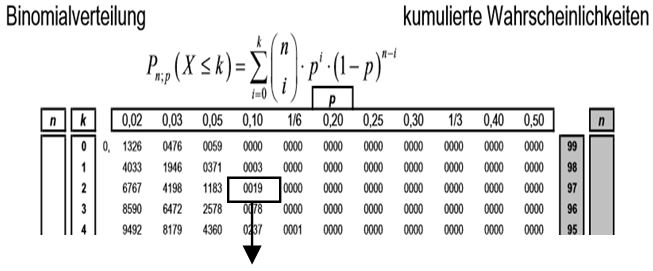
\includegraphics[width=0.48\textwidth]{../99_Bilder/04_WKR/binomtabKum.jpg}\\
		\underline{Beispiel}: Die Wahrscheinlichkeit, dass es bei einem $\ldots$-stufigen Bernoulli-Experiment mit einer Trefferwahrscheinlichkeit von \(0,10\) zu höchstens (genau oder weniger als) 2 Treffern kommt, liegt bei \(0,0019\).\\
		\subsection{Typische Gestalt der Binomialverteilung}
		Stellt man die Wahrscheinlichkeitsverteilung bei großen Werten für n als Balkendiagramm dar, ergibt sich folgendes typisches Aussehen:\\
		\par\noindent
		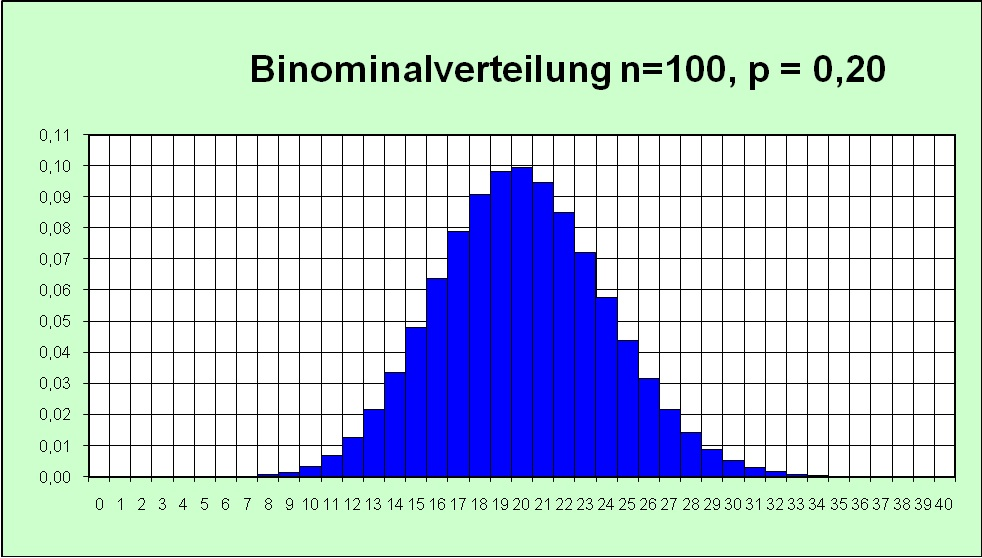
\includegraphics[width=0.48\textwidth]{../99_Bilder/04_WKR/binomBalk.jpg}\\
		\par\noindent
		Beobachtung: Es liegt eine gewisse Symmetrie vor, dort gibt es den höchsten Wahrscheinlichkeitswert. Er liegt bei \(n\cdot{}p\).
	\end{worksheet}
\end{document}